\NeedsTeXFormat{LaTeX2e}[2005/12/01]
%%    2009/03/12 v1.0 GAUBM Vorlage f�r Aschlussarbeiten Physik
%% Template fuer Bachelor- und Masterarbeiten
%% an der Fakultaet fuer Physik (c) Thomas Pruschke der GA Universit�t
%% Verbesserungsvorschlaege bitte an studiendekanat@physik.uni-goettingen.de
%%
%% Benoetigte Pakete: datenumber
%%

%%%%%%%%%%%%%%%%%%%%%%%%%%%%%%%%%%%%%%%%%%%%%%%%%%%%%%%%%%%%%%%%%%%%%%
%%%%%%%%%% Bitte vor dem Veraendern diese Datei umbenennen! %%%%%%%%%%
%%%%%%%%%%%%%%%%%%%%%%%%%%%%%%%%%%%%%%%%%%%%%%%%%%%%%%%%%%%%%%%%%%%%%%

%% scrbook - Ersatz f�r LaTeX book Klasse aus dem KOMA Script
%% Moegliche Optionen: diejenigen der Klasse scrbook ausser titlepage

%% deutsche Arbeit:
\documentclass[master,       %% Typ der Arbeit: bachelor oder master
               twoside,        %% zweiseitiges Layout
               BCOR10mm,       %% Bindekorrektur 10 mm
%               liststotoc,nomtotoc,bibtotoc, %% Aufnahme der div. Verzeichnisse
                                              %% ins Inhaltsverzeichnis
               english,ngerman, %% Alternativspr. Englisch, Dokumentspr. Deutsch
%               ngerman,english  %% Alternativspr. Deutsch, Dokumentspr. Englisch
%               final,          %% Endversion; draft fuer schnelles Kompilieren
               ]{GAUBM}

\usepackage{babel}[ngerman]
\usepackage{setspace}  %% Zur Setzung des Zeilenabstandes
%\usepackage{babel}     %% Sprachen-Unterstuetzung
\usepackage{calc}      %% ermoeglicht Rechnen mit Laengen und Zaehlern
\usepackage[T1]{fontenc}       %% Unterstutzung von Umlauten etc.
%\usepackage[latin1]{inputenc}  %%
%% in aktuellem Linux & MacOS X wird standardmaessig UTF8 kodiert!
\usepackage[utf8]{inputenc}    %% Wenn latin1 nicht geht ...

\usepackage{amsmath,amssymb} %% zusaetzliche Mathe-Symbole

\usepackage{lmodern} %% type1-taugliche CM-Schrift als Variante zur
                     %% "normalen" EC-Schrift
%% Paket fuer bibtex-Datenbanken
\usepackage[comma,numbers,sort&compress]{natbib}
\bibliographystyle{plainnat}

\newcommand{\tabheadfont}[1]{\textbf{#1}} %% Tabellenkopf in Fett
\usepackage{booktabs}                      %% Befehle fuer besseres Tabellenlayout
\usepackage{longtable}                     %% umbrechbare Tabellen
\usepackage{array}                         %% zusaetzliche Spaltenoptionen

%% umfangreiche Pakete fuer Symbole wie \micro, \ohm, \degree, \celsius etc.
%\usepackage{textcomp,gensymb}

%\usepackage{SIunits} %% Korrektes Setzen von Einheiten
%\usepackage{units}   %% Variante fuer Einheiten

%% Hyperlinks im Dokument; muss als eines der letzten Pakete geladen werden
\usepackage[pdfstartview=FitH,      % Oeffnen mit fit width
            breaklinks=true,        % Umbrueche in Links, nur bei pdflatex default
            bookmarksopen=true,     % aufgeklappte Bookmarks
            bookmarksnumbered=true  % Kapitelnummerierung in bookmarks
            ]{hyperref}

%% Weiter benoetigte Pakete: datenumber
%% Falls dieses Paket nicht in der Installation vorhanden ist,
%% kann es von der Seite mit diesem Template heruntergeladen werden
%% und in einem LaTeX bekanntem Verzeichnis installiert werden (notfalls
%% dem Verzeichnis mit der Arbeit).

\usepackage{tikz}
\usepackage{pgfplots}
\usepackage{float}

\begin{document}
%%
%%                   Ab hier muessen die Anpassungen geschehen
%%
%% Hier den eigenen Namen einsetzen
\ThesisAuthor{Anna-Jana}{Riess}
%% Hier den Geburtsort einsetzen
\PlaceOfBirth{Hamburg}
%% Titel Arbeit. Das erste Argument ist der deutsche, das zweite der
%% englische Titel.
\ThesisTitle{Spontane Axion-Leptogenese mit Generischen Kopplungen in ALP Realignment, Clockwork Axion und Multi Axion Modellen}{Spontaneous Axion-Leptogenesis with Generic Couplings in ALP Realignment, Clockwork Axion and Multi Axion Models}
%% Erst- und Zweitgutacher/in
%% Ist der/die Betreuer/in nicht identisch mit dem/r Erstgutachter/in,
%% muss diese/r als optionales Argument angegeben werden.
\FirstReferee{Prof.\ Dr.\ Laura Covi}
\Institute{Institut f\"ur Theoretische Physik}
\SecondReferee{Prof.\ Dr.\ David J. E. Marsh}
%% Beginn und Ende des Anfertigungszeitraumes
\ThesisBegin{1}{2}{2021}
\ThesisEnd{15}{8}{2022}
%% DO NOT TOUCH THESE LINES!!!!
\frontmatter
\maketitle
\cleardoublepage
%% So laesst sich in die andere Sprache umschalten (Englisch bzw. Deutsch)
\begin{otherlanguage}{english}
\begin{abstract}
  Here the key results of the thesis may be presented in about
  half a page.
  \bigskip\par
  \noindent \textbf{Keywords:} Physics, Masters Thesis, Cosmology, The Early Universe, Reheating, Axions, Baryogenesis, Spontaneous Baryogenesis, Leptogenesis, Realignment, Clockwork Theory, String Theory Axions, Non-Linear Dynamics, Thermal Field Theory, Linear Response, Transport Equation, Numerical Simulation
\end{abstract}

%% Ende des Vorspanns
\cleardoublepage
%% Ab hier 1 1/2 facher Zeilenabstand (durch setspace-Paket)
\onehalfspacing
%% Erzeugt Inhaltsverzeichnis
\tableofcontents

%%% Hier kann man seine Bezeichnungsweisen erklaeren. Falls nicht
%%% benoetigt, bis einschliesslich \end{nomenclature} auskommentieren
%\begin{nomenclature}
%%% Fuer die Berechnung der Spaltenbreiten muss \usepackage{calc}
%%% geladen sein!
%\section*{Lateinische Buchstaben}
%\noindent
%\begin{longtable}[l]{p{0.2\textwidth}p{0.7\textwidth-6\tabcolsep}p{0.1\textwidth}}
%  \tabheadfont{Variable}&\tabheadfont{Bedeutung}&\tabheadfont{Einheit}\\\midrule\endhead
%  $A$ & Querschnittsfl"ache & $\unit{m^2}$\\
%  $c$ & Geschwindigkeit & $\unitfrac{m}{s}$
%\end{longtable}
%\section*{Griechische Buchstaben}
%\begin{longtable}[l]{p{0.2\textwidth}p{0.7\textwidth-6\tabcolsep}p{0.1\textwidth}}
%  \tabheadfont{Variable}&\tabheadfont{Bedeutung}&\tabheadfont{Einheit}\\\midrule\endhead
%  $\alpha$  & Winkel & $\unit{\degree}$; --\\
%  $\varrho$ & Dichte & $\unitfrac{kg}{m^3}$
%\end{longtable}
%\section*{Indizes}
%\begin{longtable}[l]{p{0.2\textwidth}p{0.8\textwidth-4\tabcolsep}}
%  \tabheadfont{Index}&\tabheadfont{Bedeutung}\\\midrule\endhead
%  m & Meridian\\
%  $r$ & Radial
%\end{longtable}
%\section*{Abk"urzungen}
%\begin{longtable}[l]{p{0.2\textwidth}p{0.8\textwidth-4\tabcolsep}}
%  \tabheadfont{Abk"urzung}&\tabheadfont{Bedeutung}\\\midrule\endhead
%  2D & zweidimensional\\
%  3D & dreidimensional\\
%  max & maximal
%\end{longtable}
%\end{nomenclature}
%% \listoftables und \listoffigures sollten nur bei genuegender Anzahl Tabellen
%% verwendet werden
%\listoffigures
%\listoftables

\mainmatter   %% Anfang Hauptteil

\chapter{Introduction}

MOTIVATION!!!
-> we are here, a

PROBLEM OVERVIEW

CONTENT SUMMERY OF THESIS

In this thesis we will always use natural units with $c = \hbar = k_B = 0$
and the following metric convention $(+1, -1, -1, -1)$
TODO: check metric convention everywhere!!!!!!!!!

\chapter{Fundamentals}

\section{Early Universe Cosmology}
In this section we will introduce the basics of cosmology and the background cosmological model we will use for the computations in this thesis later on.
A good reference and the source for this section is \cite{the_early_universe_kolb_and_turner}.

\subsection{Dynamics of the Expansion of the Universe}
\label{sec:dynamics_of_the_examsion_of_the_universe}
The dynamics of the expanding universe is governed by Einsteins theory of general relativity. The Einstein field-equation connects geometry i.e. the curvature with the content i.e. the energy-momentum tensor $T$ of the universe \footnote{
TODO: introduce all quantities????
}:
\begin{equation}
	R_{\mu \nu} - \frac{1}{2} R g_{\mu \nu} = 8 \pi G T_{\mu \nu}.
\end{equation}
We assume the cosmological assumption that the universe is homogeneous and isotropic on the large scales we are interested in. In this case the most general form of the metric is the Friedmann-Lametre-Robinson-Walker metric, which reads:
\begin{equation}
	\mathrm{d} s^2 = - \mathrm{d} t^2 + a(t) \left[ \frac{\mathrm{d} r^2}{1 - kr^2} + \mathrm{d} \Omega \right].
\end{equation}
The quatitiy $a$ is called the scale factor and has to be determined by the Einstein field-equations.
The parameter $k$ fixes the topology of the universe. In this thesis we use $k = 0$ i.e. a flat universe as suggested by data of e.g. the Planck mission \cite{planck2018}.
On the overhand the content of an homogeneous and isotropic universe filled with a perfect fluid, has a diagonal energy-momentum tensor given by:
\begin{equation}
	T_\nu^\mu = \operatorname{diag}(\rho, P, P, P),
\end{equation}
where $\rho$ is the energy-density and $P$ the pressure.
Plugging these assumption into the Einstein field-equations yields the Friedmann equation (first order constraint, from the $T^{00}$ component) \footnote{
A useful compact form of the Friedmann equation for $k = 0$ and $M_\mathrm{pl} = 1 / \sqrt{8 \pi G}$ is $3 M_\mathrm{pl} H^2 = \rho$
}:
\begin{equation}
	\left( \frac{\dot{a}}{a} \right)^2 = \frac{8 \pi G}{3} \rho - \frac{k}{a^2}
\end{equation}
as well as the acceleration equation (second order e.o.m., from the trace of $T$)
\begin{equation}
	\frac{\ddot{a}}{a} = - \frac{4 \pi G}{3} ( \rho + 3 p ).
\end{equation}
From these equations one can derive a continuity equation for the energy-momentum tensor
\begin{equation}
	\label{eq:continuity_equation}
	\dot{\rho} = - 3 H (\rho + P),
\end{equation}
where $H = \frac{\dot{a}}{a}$ is the Hubble-parameter. \\
\noindent A set of useful solutions for $k = $ can be derived for a power-law dependence of the energy density on the scale-factor $\rho = \rho_0 a^X$ i.e. that the dilution of the energy is described by a power-law. For this we also introduce the so called equation of state (e.o.s.)
\begin{equation}
	w = \frac{P}{\rho}.
\end{equation}
This can in general have a complicated form and depend on further parameters such as temperature or field configurations, but we will assume a constant e.o.s $w$ for now.
Then one finds using eq. \eqref{eq:continuity_equation}:
\begin{equation}
	\rho \sim a^{-3(1 + w)}.
\end{equation}
This result is important as most of the universes history falls into this case.
One finds the following relations:
\begin{align}
	p &= \frac{1}{3} \rho \implies \rho \sim a^{-4} \quad \mathrm{(Radiation)} \nonumber \\
	p &= 0 \implies \rho \sim a^{-3} \quad \mathrm{(Matter)} \nonumber \\
	p &= - \rho \implies \rho \sim \mathrm{const} \quad \mathrm{(Vacuum Energy)}
\end{align}
While matter is just diluted in numbers by the expansion, radiation is also redshifted.
Vacuum energy is essentially defined by this equation of state.
Finally we mention that energy densities is often stated relative to the critical-density $\rho_c = \frac{3 H^2}{8 \pi G}$ as
\begin{equation}
	\Omega_i = \frac{\rho_i}{\rho_c}.
\end{equation}

\subsection{Cosmological Equilibrium Thermodynamics}
We will now cover the thermodynamic description of the particle content of the universe
in equilibrium.
In this case the distribution of particles is given by Fermi-Dirac or Bose-Einstein for ferminons or bosons respectively \footnote{

}:
\begin{equation}
	f(\mathbf{p}) = \frac{1}{\exp((E - \mu) / T) \pm 1},
\end{equation}
where we have the relativistic relation for the energy $E^2 = p^2 + m^2$. The distribution is parametrized by the temperature $T$ and the chemical potential $\mu$.
Note the different sign in the expression for fermions and bosons.
From this probability distribution one can compute the important thermodynamics observables.
The number density of particles:
\begin{equation}
	n = \frac{g}{(2\pi)^3} \int \mathrm{d}^3 p f(\mathbf{p})
\end{equation}
The energy density:
\begin{equation}
	\rho = \frac{g}{(2\pi)^3} \int \mathrm{d}^3 p E(\mathbf{p}) f(\mathbf{p})
\end{equation}
The pressure:
\begin{equation}
	p = \frac{g}{(2\pi)^3} \int \mathrm{d}^3 p \frac{p^2}{3E(\mathbf{p})} f(\mathbf{p})
\end{equation}
These integrals can be evaluated in the relativistic limit where $m \ll T$:
\begin{equation}
	\rho = \begin{cases}
		\frac{\pi^2}{30} g T^4 & \text{Bosons} \\
		\frac{7}{8} \frac{\pi^2}{30} g T^4 & \text{Fermions}
	\end{cases}
\end{equation}
\begin{equation}
	n = \begin{cases}
		\frac{\zeta(3)}{\pi^2} g T^3 & \text{Bosons} \\
		\frac{3}{4} \frac{\zeta(3)}{\pi^2} g T^3 & \text{Fermions}
	\end{cases}
\end{equation}
\begin{equation}
	p = \rho / 3
\end{equation}
\begin{equation}
	s = \frac{2 \pi^2}{45} g_i T^3
\end{equation}

\begin{equation}
	n_+ - n_- \approx \frac{g T^3}{6} \left( \frac{\mu}{T} \right)
\end{equation}

This result can be generalized to multiple particle species by using effective degrees of freedom $g_*$:
\begin{align}
	\rho &= \frac{\pi^2}{30} g_{*, \rho}(T) T^4 \nonumber \\
	s &= \frac{2 \pi^2}{45} g_i T^3
\end{align}
with
\begin{equation}
	g_{*, \rho} = \sum_{i, \text{bosons}} g_i \left( \frac{T_i}{T} \right)^4 + \frac{7}{8} \sum_{i, \text{fermions}} g_i \left( \frac{T_i}{T} \right)^4
\end{equation}
and for the entropy:
\begin{equation}
	g_{*, s} = \sum_{i, \text{bosons}} g_i \left( \frac{T_i}{T} \right)^3 + \frac{7}{8} \sum_{i, \text{fermions}} g_i \left( \frac{T_i}{T} \right)^3.
\end{equation}
These expressions allow us to model the standard model plasma in the early universe, if
all interactions are fast enough.


\subsection{Inflation and Reheating}
In order to solve several problems with standard Friedmann cosmology as discussed so far e.g. the flatness problem i.e. the fine-tuning of $k = 0$,
an epoch of exponential expansion before the usual subsequent evolution of the universe is proposed. The easiest way to implement this, is so called slow-roll inflation. In this model a scalar field called the inflaton field $\phi$ with a mass $m_\mathrm{inf}$ is introduced. The equation of motion for the inflaton field reads \footnote{see section \ref{sec:motion_of_the_axion_field} for the derivation of equation of motion of scalar fields in a expanding universe.}:
\begin{equation}
	\label{eq:inflaton_field_eq}
	\ddot{\phi} + 3 H \dot{\phi} + \Gamma_\mathrm{inf} \dot{\phi} + V'(\phi) = 0.
\end{equation}
The energy density is given by the energy density of the inflaton field
and standard model radiation:
\begin{align}
	\rho_\mathrm{inf} &= \frac{1}{2} \dot{\phi}^2 + \frac{1}{2} m_\mathrm{inf}^2 \phi^2 \\
	\rho &= \rho_\mathrm{inf} + \rho_\mathrm{rad}.
\end{align}
TODO: describe initial condition for reheating
\begin{align}
	\rho_\mathrm{inf}(t_\mathrm{inf}) &= 3 M_\mathrm{pl}^2 H_\mathrm{inf}^2 \nonumber \\
	\rho_\mathrm{rad}(t_\mathrm{inf}) &= 0
\end{align}
The term $\Gamma_\mathrm{inf}$ is a phenomenological term describing the decay of the inflaton field into standard model particles, as we will see shortly. In this thesis we are interested in the epoch after the inflaton starts oscillating and decays into standard model particles. This epoch is called reheating.
If we multiply eq. \eqref{eq:inflaton_field_eq} with $\dot{\phi}$ and average over one oscillation, we obtain
the equation for reheating:
\begin{equation}
	\dot{\rho}_\mathrm{inf} + 3 H \rho_\mathrm{inf} = - \Gamma_\mathrm{inf} \rho_\mathrm{inf}
\end{equation}
The corresponding equation for the radiation energy density reads
\begin{equation}
	\dot{\rho}_\mathrm{rad} + 4 H \rho_\mathrm{rad} = + \Gamma_\mathrm{inf} \rho_\mathrm{inf}
\end{equation}
The replacement $4 \to 3$ comes from the different scaling of the energy density from the expansion. The change of sign on the right-hand-side comes from the direction of the decay. Here one can see the effect of the $\Gamma_{\mathrm{inf}}$: it creates an effective decay term in the rate equations.
These equations together with the Friedmann equation, describe the background cosmology for our later computations.

\section{Axions}
TODO: do we need this paragraph????
In this section we will review axion-like particles, starting and considering QCD-axions as our example. For this we will follow the review \cite{Di_Luzio_2020_Landscape_of_QCD_Axion_models}.
The theory of QCD contains a term call the theta term:






\section{Baryogenesis}
In this section we will introduce the problem for which this thesis investigates a possible solution.
The problem of baryogenesis can be expressed as follows: Why does the universe contain so much baryonic-matter? Or more precise: The universe as observed today, is made up of matter with very little antimatter, while in earlier times both were present in high numbers being in chemical equilibrium. As the universe cooled down, most of matter and antimatter annihilated into photons. Therefore it is reasonable to express the amount of matter-antimatter asymmetry by the ratio of the effective baryon number and the number of photons:
\begin{equation}
	\eta_B = \frac{n_+ - n_-}{n_\gamma},
\end{equation}
with
\begin{equation}
	n_\gamma = 2 \frac{\zeta(3)}{\pi^2} T^3.
\end{equation}
The dependence on the expansion in $\eta_b$ cancels out.
Only a comparatively small number of baryons survived in the end.
For lower energies we know that baryon number is a conserved quantity. Hence the creation of the asymmetry needs to happen at high energies.
Note that during annihilation of baryons and antibaryons ??? the comoving number of photons changes, hence over this epoch the asymmetry $\eta_B$ is not conversed. A better quantifier for the baryon-asymmetry
is the ratio with the entropy density:
\begin{equation}
	\label{eq:baryon_abundance}
	Y_B := \frac{n_B}{s}.
\end{equation}
The present-day asymmetry in relation to the photons number density can be expressed as \footnote{
One can derive this by considering $\frac{\eta_B}{Y_B} = \frac{\pi^4}{45 \zeta(3)} g_{*, s}(T)$.
In the standard model one finds $g_{*,s}^0 = 43/11$ and $g_{*, s}^{\gg 1 \, \mathrm{Gev}} = 427/4$ \cite[sec. 3.4]{the_early_universe_kolb_and_turner}.
}
\begin{equation}
	\eta_B^0 = \frac{g_{*,s}^0}{g_{*, s}^{\gg 1 \, \mathrm{Gev}}} \eta_B^{\gg 1 \, \mathrm{Gev}}.
\end{equation}

\subsection{Sakharov Conditions}
Andrei Sakharov formulated in 1967 three necessary conditions required for baryogenesis \cite{Sakharov_1991}.
The first is that baryon number has to be violated in the process. We start from the assumption that the initial baryon asymmetry was vanishing as it was diluted by inflation.
Hence the baryon number as to the violated in a dynamical process.
The second one is less obvious: C and CP symmetries have to be broken.
This is required as only if
reactions exists that actually biased toward the creation of baryons not anti-baryons an effective asymmetry can be produced.
For this to happen the reactions need to distinguish between matter and antimatter i.e. C and CP symmetries have a be broken.
Finally the process of baryogenesis has to happen out-of-equilibrium. This is because
in equilibrium the number densities only depend on the mass of the particles, which is the same of particles and their anti-partners.


\subsection{Baryogenesis in the Standard Model}
\label{sec:baryogenesis_in_the_standard_model}

Let us investigate these conditions in the known physics of the standard model (SM). While non-equilibrium and C / CP violation are know parts of the standard model, baryon number violation do not appear in the Feynman rules of SM interaction. In the standard model, the baryon and the lepton numbers are violated by the following non-perturbative term:
\begin{equation}
	\label{eq:B_and_L_current_equations}
	\partial_\mu J^\mu_B = \partial_\mu J^\mu_L = N_f \frac{g_2^2}{32 \pi^2} F^{\mu \nu}_a \tilde{F}_{\mu \nu}^a,
\end{equation}
where $g_2$ is the SU(2) coupling constant, $N_f$ the number of fermions, $F$ the SU(2) field strength tensor and $\tilde{F}$ its dual.
It can be written as the divergence of the Chern-Simons current:
\begin{equation}
	\label{eq:chern_simons_current}
	K^\mu = \epsilon^{\mu \alpha \beta \gamma} \left( A^a_\alpha F^a_{\beta \gamma} - \frac{g_2}{3} f^{abc} A^a_\alpha A^b_\beta A^c_\gamma \right),
\end{equation}
where $f^{abc}$ are the SU(2) structure constants, $A$ the SU(2) gauge field.
This shows that the term on the right hand side of \eqref{eq:B_and_L_current_equations} is a topological quantity as we can define a winding-number type quantity:
\begin{equation}
	N_{\mathrm{CS}} := \int \mathrm{d}^3 x \, K^0.
\end{equation}
Using the temporal gauge defined by $A_0 = 0$, where $K_i = 0$,
we can write the change of Chern-Simons number between $t_i$ and $t_f$ as
\begin{equation}
	\int \mathrm{d}^4 x \partial_\mu K^\mu = \int \mathrm{d} t \, \partial_t \int \mathrm{d}^3 x \, K^0 =
	N_{\mathrm{CS}}(t_f) - N_{\mathrm{CS}}(t_i) = \Delta N_{\mathrm{CS}}(t_i, t_f)
\end{equation}
If the field configurations at $t_i$ and $_f$ are so called pure gauges i.e. configurations with vanishing energy-density (vaccum configurations) and hence vanishing field strength of the form
\begin{equation}
	A_\mu = U^{-1} A_\mu U + \frac{i}{g_2} U^{-1} \partial_\mu U,
\end{equation}
then the Chern-Simons number is an integer.
Hence one can not deform such vacuum configurations into each other without leaving the set of vacuum configurations.
The change between them is hence a quantum tunneling process called an instanton \footnote{TODO: explain formal defintion of instanton}. See figure \ref{fig:sphaleron_cartoon} for an illustration.
Its rate is too low to have any significant effect, although this changes once we consider thermal processes i.e. so called sphalerons \footnote{TODO: explain sphaleron configurations}.
Below the electro-weak phase transition the rate is still exponentially suppressed but the energy barrier between vaccua vanishes above the phase transition. Here the transition rate is given by
\begin{align}
	\Gamma_{\mathrm{sph}} &= (0.21 \pm 0.01) \left(\frac{N_c g^2 T}{m_D^2} \right) \left(\ln \left(\frac{m_D}{\gamma} \right) + 3.0410 \right) \frac{N_c^2 - 1}{N_c^2} (N_c \sqrt{2 \pi g})^5 T^4 \\
	\gamma &= \frac{N_c g^2 T}{4 \pi} \left(\ln \left(\frac{m_D}{\gamma}\right) + 3.0410 \right) \nonumber \\
	m_D^2 &= \frac{2N_c + N_f}{6} g^2 T^2 \nonumber,
\end{align}
where $N_c$ the number of ``colors'' ($N_c = 2$ for the weak SU(2) theory) and $g = g_2$ the coupling constant.
These processes give us the rate of conversion of lepton and baryon numbers.

\begin{figure}[H]
	\centering
	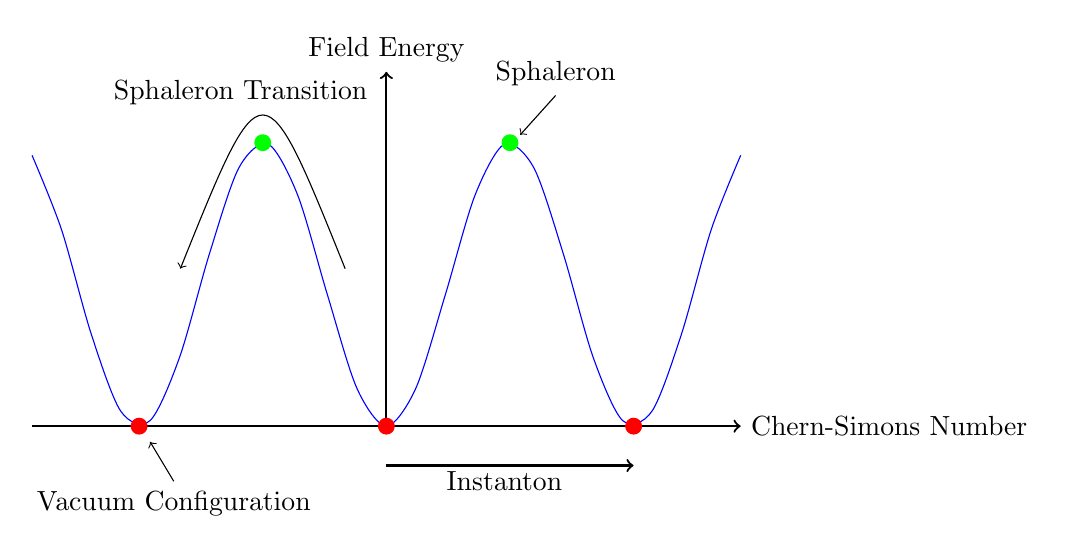
\begin{tikzpicture}
		\draw[thick,->] (-4.5,0) -- (4.5,0) node[anchor=west] {Chern-Simons Number};
		\draw[thick,->] (0,0) -- (0,4.5) node[anchor=south] {Field Energy};
		\draw[scale=1, domain=-4.5:4.5, smooth, variable=\x, blue] plot ({\x}, {1.8*(1 - cos(2 * \x r))});
		\foreach \x in {0,3.14,-3.14}
		\filldraw[color=red] (\x, 0) circle (0.1);
		\foreach \x in {3.14/2, -3.14/2}
		\filldraw[color=green] (\x, 1.8*2) circle (0.1);
		\draw[thick,->] (0.0, -0.5) -- (3.14, -0.5);
		\draw[->] (3.3 / 2 + 0.5, 1.8*2 + 0.5 + 0.1) node[anchor=south]  {Sphaleron} -- (3.4 / 2, 1.8*2 + 0.1) ;
		\draw[->] (-2.7, -0.7) node[anchor=north]  {Vacuum Configuration} -- (-3, -0.2) ;
		\node at (1.5, -0.7) {Instanton};
		\draw[->] (-3.14/6, 2) .. controls (-3.14 / 2, 1.8*2 + 1) .. (-3.14 + 3.14/6, 2) node[midway,above,xshift=-8]{Sphaleron Transition};
	\end{tikzpicture}
	\caption{Cartoon of the vacuum structure of a non-albelian gauge theory, which leads to the non-conservation of baryon and lepton numbers in the standard model.
		On the x-axis the Chern-Simons number is shown and on the y-axis the free-energy of the gauge field.
		The energy is sketched as a blue line. The vacuum-configurations are indicated by red dots and the sphaleron configurations by green ones. Sphaleron and instanton transitions are indicated by arrows from one vacuum state
		to the next.
	}
	\label{fig:sphaleron_cartoon}
\end{figure}


\chapter{Spontaneous Baryogenesis}
In this chapter we will discuss a possible mechanism which could implement baryogenesis. This mechanism is call spontaneous baryogenesis and is the topic of the rest of this thesis.

\section{Mechanism of Spontaneous Baryogenesis}

The mechanism of spontaneous baryogenesis was propose by Andreq Cohen and David Kapla in 1987 in \cite{COHEN1987251} and \cite{COHEN1988913}.
Their idea was to couple a scalar field $\phi$ to the baryon current $J_B$:
\begin{equation}
	\mathcal{L} = \frac{1}{2} (\partial \phi)^2 - V(\phi) - \frac{1}{f} \partial_\mu \phi J_B^\mu.
\end{equation}
If one considers the corresponding path-integral for the thermal theory, the time derivative in this coupling appears as a modification of the baryon chemical potential:
\begin{equation}
	\mu \to \mu_\mathrm{eff} = \mu + \frac{\dot{\phi}}{f}.
\end{equation}
This in turn modifies the equilibrium abundance of baryons, depending on the sign of $\dot{\phi}$.
In a cosmological setting, a scalar field is frozen until its mass exceeds the Hubble-friction (see \ref{sec:motion_of_the_axion_field} for details on this). The initial fast-roll motion creates baryons. Then the successive oscillations create baryons and antibaryons in alternation canceling each other, without creating a net baryon number.
There are different ways to create an concrete implementation of spontaneous baryogenesis.
The one we will look at in this thesis is using axions.
Axions have couplings the topological terms like
\begin{equation}
	 \sim \phi(t) F \tilde{F}.
\end{equation}
From eq. \eqref{eq:B_and_L_current_equations} we can see that this creates a direct coupling to the lepton current.
Then, by the means of sphalerons (see section \ref{sec:baryogenesis_in_the_standard_model}), the leptons are converted into baryons.

In ref. \cite{Domcke:2020kcp_Generic_Couplings} the authors pointed out that a direct coupling to the lepton or baryon current is not necessary for successful baryogenesis.
Instead the creation of some charge X deviating from the equilibrium value, leeds to a non-vanishing baryon number if the reactions which equilibrate the charge X back, are violating baryon number. Hence in the process a net baryon number is created.
Let us discuss this on an abstract example in more detail.
We are considering two charges $Q_1$ and $Q_2$. The baryon number is given by the linear combination
\begin{equation}
	B = Q_1 + Q_2.
\end{equation}
Our toy theory contains two interactions: $O_1$, which changes $Q_1$ by $-1$ and $Q_2$ by $+1$ and $O_2$, which changes $Q_1$ by $+1$. In equations, the current equations for this theory are:
\begin{align}
	\partial_\mu J_1^\mu &= O_2 - O_1 \\
	\partial_\mu J_2^\mu &= O_1 \nonumber.
\end{align}
Hence the current equation for the baryon current reads
\begin{equation}
	\partial_\mu J_B^\mu = O_2.
\end{equation}
The mechanism discussed so far would work by coupling the scalar field to the operator $O_2$, leading to a direct coupling of the scalar field to the baryon current. But in this example we couple it to $O_1$.
This coupling biases the value of $Q_2 - Q_1$ away from the previous vanishing equilibrium value.
At the same time, the the operator $O_2$ will lead to a relaxation of $Q_1$ toward its vanishing equilibrium value. In doing so it will violate also $B = Q_1 + Q_2$ as it doesn't change $Q_2$. Once this reaction freezes out, $B$ is conserved. Then $O_2$ will lead $Q_2 - Q_1$ to obtain its new vanishing equilibrium value with a non-vanishing $B$.
A cartoon of this process is shown in fig. ????? TODO

Why is this process called \emph{spontaneous} baryogenesis?
This is because the amount and also if baryons or antibaryons are generated depends on the initial value of the scalar field.
If in the UV-completion this scalar arises as the (pseudo-)Goldstone boson of the spontaneous symmetry breaking (SSB) of a complex field $\Phi$, then the initial values of $\phi$ are distributed evenly from the SSB, hence the name spontaneous baryogenesis.

Finally we have to find a way to compute the final asymmetry.
A simple approach is using Boltzmann equations. For example if we couple
the axion field directly to the lepton current and we have lepton number violating interaction in the thermal plasma mediated by the Weinberg operator
\begin{equation}
	???????
\end{equation}
then the Boltzmann equation reads:
\begin{equation}
	??????
\end{equation}
This equation was used in ref. \cite{Kusenko_2015_Axion_Leptogenesis}.
However we would like to have a complete set of equations considering all standard model charges. The equation above assumes that these charges are all in equilibrium.
Moreover this approach has the problem that it depends on the field basis.
This problem was pointed out by ref. \cite{Shi_2015_Basis_Invariance_chemical_equilibrium}.
If we would start with an axion coupling to the weak sphaleron $a F \tilde{F}$, this Boltzmann equation is not correct. As this coupling is not directly modifying the lepton chemical potential. For this one needs a coupling to the lepton current.
To introduce a coupling to the lepton current from this coupling, one needs to do a field redefinition depending on the axion field. This would also change the fields in the Weinberg operator, introducing a coupling within the Weinberg operator, modifying its rate. While one could compute a rate for the Weinberg operator including the axion dependence and solve for the asymmetry correctly, its more fruitful to use a set of basis independent equations.
This was done in .ref \cite{Domcke:2020kcp_Generic_Couplings}, where the authors developed a formalism based on linear-response theory which can describe the equilibration of charges by interaction and generation of charges from coupling to an axion field in a basis independent way for generic couplings. We will now recap their derivation.

\section{Transport Equation I: Derivation}
The following derivation of the transport equation is taken from  \cite[appendix B]{Domcke:2020kcp_Generic_Couplings}.

We start from the current (continuity) equation for the charges $Q_i$ with current $J_i^\mu$. These charges are changed by interaction $O_\alpha$ by $n_i^\alpha$:
\begin{equation}
	\label{eq:current_eq}
	\partial_\mu J_i^\mu = \sum_\alpha n_i^\alpha O_\alpha
\end{equation}
This equation is directly derived from the Lagrangian of the system and should be taken as an operator valued equation in the context of finite temperature QFT. We are working in the Heisenberg picture, where the states and the density matrix do not evolve with time but the observables do.
We want to take the expectation value in the grand-canonical ensemble as particle numbers are not conserved:
\begin{equation}
	\label{eq:current_eq_expectation_value}
	\partial_t \langle J_i^0 \rangle_{\mathrm{GC}} = \sum_\alpha n_i^\alpha \langle O_\alpha \rangle_{\mathrm{GC}}
\end{equation}
We are going to evaluate these expectation values in linear-response theory.
For this we take $H_s \equiv \sum_i \mu_i Q_i$ as a perturbation to the Hamiltonian of the system.
Here the $\mu_i$ are the sources, which change slowly compared to the charges $Q_i$.
Let us first derive the equation for linear perturbation theory in general and then apply is first to the perturbation by chemical potentials $\mu_i$ and then to the perturbation by the classical axions field $a(t)$.
We work in the interaction-picture, where the time-evolution of the density matrix $\rho(t)$ of the system is given by
\begin{equation}
    \rho(t) = U(t) \rho_0 U^{-1}(t).
\end{equation}
The interaction-picture time-evolution operator $U(t)$ is given by
\begin{equation}
    U(t) = T \, \exp \left[ - i \int_{-\infty}^t  \mathrm{d} t' H_s(t') \right].
\end{equation}
We now evaluate an arbitrary observable $A_i$ with this density matrix in linear order of perturbation theory:
\begin{align}
	\label{eq:linear_response}
    \langle A_i \rangle &= \operatorname{Tr} \left[ \rho(t) A_i(t) \right] \nonumber \\
    &= \operatorname{Tr} \left[ U(t) \rho_0 U^{-1}(t) A_i(t) \right] \nonumber \\
    &= \operatorname{Tr} \left[ \rho_0 U^{-1}(t) A_i(t) U(t) \right] \nonumber \\
    &\approx \operatorname{Tr} \left[ \rho_0 (1 + i \int_{-\infty}^t \mathrm{d} t' H_s(t')) A_i(t) (1 - i \int_{-\infty}^t \mathrm{d} t' H_s(t')) \right] \nonumber \\
    &\approx \operatorname{Tr} \left[ \rho_0 (A_i(t) + i \int_{-\infty}^t \mathrm{d} t' [H_s(t'), A_i(t)] ) \right] \nonumber \\
    &= \langle A_i \rangle_c + i \int_{-\infty}^t \mathrm{d} t' \langle [H_s(t'), A_i(t)] \rangle_c \nonumber \\
    &= \langle A_i \rangle_c + i \int_{-\infty}^t \mathrm{d} t' \langle [\sum_j \phi_j(t') A_j(t'), A_i(t)] \rangle_c  \nonumber \\
    &= \langle A_i \rangle_c + i \sum_j \int_{-\infty}^t \mathrm{d} t' \phi_j(t') \langle [A_j(t'), A_i(t)] \rangle_c
\end{align}

Now we can apply this to the chemical potentials.
We want to take the exception values of the interaction operators $O_\alpha$ in eq. \eqref{eq:current_eq_expectation_value}.
Here the chemical potentials $\mu_i$ are the sources and they are coupled to the charges $Q_i$.
Hence the linear response equations reads
\begin{equation}
	\langle O_\alpha(t, x) \rangle = i \sum_j \int_{-\infty}^t \mathrm{d} t' \mu_j(t') \langle [Q_j(t'), O_\alpha(t, x)] \rangle_c.
\end{equation}
Here we have used that $\langle O_\alpha(t) \rangle_c = 0$.
Now we are going to insert the charges in terms of the time component of the four-current:
\begin{equation}
	Q_i(t) = \int \mathrm{d}^3 x J^0_i(t, x)
\end{equation}
and insert a dummy integration to write the equation in terms of the time derivative of the charge density $\dot{J^0_i}$ and finally replace it with the right-hand-side of the current eq. \eqref{eq:current_eq}:
\begin{align}
	\langle O_\alpha(t, x) \rangle &= i \sum_j \int_{-\infty}^t \mathrm{d} t' \mu_j(t') \langle [\int \mathrm{d}^3 x' J^0_j(t', x'), O_\alpha(t, x)] \rangle_c \nonumber \\
	&= i \sum_j \int_{-\infty}^t \mathrm{d} t' \int \mathrm{d}^3 x'  \mu_j(t') \langle [\int^{t'}_{-\infty} \ \mathrm{d} t'' \frac{\partial}{\partial t''} J^0_j(t'', x'), O_\alpha(t, x)] \rangle_c \nonumber \\
	&= i \sum_j \int_{-\infty}^t \mathrm{d} t' \int \mathrm{d}^3 x'  \mu_j(t') \langle [\int^{t'}_{-\infty} \ \mathrm{d} t'' \sum_\beta n^\beta_j O_\beta(t'', x'), O_\alpha(t, x)] \rangle_c \nonumber \\
	&= i \sum_{j, \beta} \int_{-\infty}^t \mathrm{d} t' \int \mathrm{d}^3 x' \int^{t'}_{-\infty} \ \mathrm{d} t'' \mu_j(t') n^\beta_j \langle [ O_\beta(t'', x'), O_\alpha(t)] \rangle_c
\end{align}
Finally we use the assumption that the chemical potentials change slowly compared to the charges
\begin{equation}
	\langle O_\alpha(t, x) \rangle = i \sum_{j, \beta} \mu_j(t) n^\beta_j  \int_{-\infty}^t \mathrm{d} t' \int \mathrm{d}^3 x' \int^{t'}_{-\infty} \ \mathrm{d} t'' \langle [ O_\beta(t'', x'), O_\alpha(t, x)] \rangle_c.
\end{equation}
This equation can now be expressed in terms of the spectral functions
\begin{equation}
	G_{\alpha \beta}(t - t', x - x') \equiv \langle [ O_\alpha(t, x), O_\beta(t', x')] \rangle_{c}
\end{equation}
\begin{equation}G_{\alpha \beta}(\omega, p) \equiv \int \mathrm{d}^3 x \, \mathrm{d} t \, e^{i \omega t - i p \cdot x} G_{\alpha, \beta}(t, x)
\end{equation}
\begin{equation}G_{\alpha \beta}(t, x) = \int \frac{\mathrm{d}^3 p \, \mathrm{d} \omega}{2 \pi} \, e^{- i \omega t + i p \cdot x} G_{\alpha \beta}(\omega, p).
\end{equation}
as
\begin{equation}
	\langle O_\alpha(t, x) \rangle = i \sum_{j, \beta} \mu_j(t) n^\beta_j  \int_{-\infty}^t \mathrm{d} t' \int \mathrm{d}^3 x' \int^{t'}_{-\infty} \ \mathrm{d} t'' G_{\alpha \beta}(t - t'', x - x')
\end{equation}
\begin{equation}
	\langle O_\alpha(t) \rangle = i \sum_{j, \beta} \mu_j(t) n^\beta_j  \int_{-\infty}^t \mathrm{d} t' \int \mathrm{d}^3 x' \int^{t'}_{-\infty} \ \mathrm{d} t''
	\int \frac{\mathrm{d}^3 p \, \mathrm{d} \omega}{2 \pi} \, e^{- i \omega (t - t'') + i p \cdot x'} G_{\alpha \beta}(\omega, p).
\end{equation}
We are now going to evaluate most of the integrals in this expression. Here we are commiting some crimes against maths! First we use the cancellations between the $x$ and the $p$ integrals and then isolate and finally solve the $t$ integrals:
\begin{align}
	& \int_{-\infty}^t \mathrm{d} t' \int \mathrm{d}^3 x' \int^{t'}_{-\infty} \ \mathrm{d} t''
	\int \frac{\mathrm{d}^3 p \, \mathrm{d} \omega}{2 \pi} \, e^{- i \omega (t - t'') + i p \cdot x'} G_{\alpha \beta}(\omega, p) \nonumber \\
	= & \int \frac{\mathrm{d} \omega}{2 \pi} G_{\alpha \beta}(\omega, 0) \int_{-\infty}^t \mathrm{d} t' \int^{t'}_{-\infty} \ \mathrm{d} t''
	\, e^{- i \omega (t - t'')}  \nonumber \\
	= & - \int \frac{\mathrm{d} \omega}{2 \pi} \frac{G_{\alpha \beta}(\omega, 0)} {\omega^2}
\end{align}
Plugging this back into the expression for the expectation value yields:
\begin{equation}
	\langle O_\alpha(t) \rangle = \sum_{j, \beta} \mu_j(t) n^\beta_j \int \frac{\mathrm{d} \omega}{2 \pi} \frac{G_{\alpha \beta}(\omega, 0)} { \omega (\omega + i \epsilon)} =  \sum_{j} \mu_j(t) n^\alpha_j \frac{G_{\alpha \alpha}(\omega, 0)}{2 \omega} \Big|_{w = 0}.
	\label{eq:chemical_potentials_linear_response}
\end{equation}
Here we have used that 
\begin{equation}
	\int_{-\infty}^{+\infty} \frac{\mathrm{d} \omega}{2\pi i} \frac{1}{\omega^2} G_{\alpha \beta}(\omega, 0) = \frac{1}{2} \int_l \frac{\mathrm{d} \omega}{2\pi i} \frac{1}{\omega} \frac{G_{\alpha \beta}(\omega, 0)}{\omega} = \frac{G_{\alpha \beta}(\omega, 0)}{2 \omega} \Big|_{\omega = 0} \underbrace{\operatorname{Res}_{\omega = 0} \frac{1}{\omega}}_{= 1},
\end{equation}
where $l$ is the contour from $+\infty$ to zero and back.

Now we turn to the source from the axion field $a(t)$.
This time our perturbation Hamiltonian reads
\begin{equation}
	H_s(t) = \frac{a(t)}{f_a} \int \mathrm{d}^3 x \, O_\beta(t, x).
\end{equation}
We again use eq. \eqref{eq:linear_response} to obtain the linear response result
\begin{equation}
	\langle O_\alpha(t) \rangle_{GC, a \ne 0} = \langle O_\alpha \rangle_{GC, a = 0} + i \int_{-\infty}^t \mathrm{d}^4 x' \frac{a(t')}{f_a} \langle [ O_\beta(x'), O_\alpha(x)] \rangle_c.
\end{equation}
Note that the expectation values with the GC (grand-canonical ensemble) subscript are taken using the linear response result with the chemical potentials.
Finally we use the assumption that the axion field changes slowly compared to the charges. In this case we are allowed to expand the axion field
around time $t$ as
\begin{equation}
	a(t') = a(t) + \dot{a}(t)(t' - t).
\end{equation}
This yields:
\begin{align}
	 &\langle O_\alpha(t) \rangle_{GC, a \ne 0} - \langle O_\alpha  \rangle_{GC, a = 0} = - i \frac{a_0}{f_a} \int_{-\infty}^t \mathrm{d}^4 x' G_{\alpha \beta}(x') - i \frac{\dot{a}}{f_a} \int_{-\infty}^t \mathrm{d}^4 x' G_{\alpha \beta}(x') (t - t')
	 \nonumber \\ 
	 &= - \frac{a_0}{f_a} \int_{-\infty}^t \mathrm{d} t' \int \mathrm{d} \omega \frac{e^{i \omega (t - t') - i p x'}}{(2\pi)^4} G_{\alpha \beta}(\omega, 0)
	 -i \frac{\dot{a}_0}{f_a} \int_{-\infty}^t \mathrm{d} t' \underbrace{\int \frac{\mathrm{d} \omega}{2 \pi} G_{\alpha \beta}(\omega, 0) \underbrace{(t - t') e^{i \omega (t - t')}}_{= -i \partial_\omega e^{i \omega (t - t')}}}_{= - \int \mathrm{d} \omega \partial_\omega G_{\alpha \beta}(\omega, 0) e^{i \omega (t - t')}}
	 \nonumber \\
	 &= - \frac{a_0}{f_a} \int \mathrm{d} \omega \frac{1}{2 \pi \omega} G_{\alpha \beta}(\omega, 0) - i \frac{\dot{a}_0}{f_a} \int \mathrm{d} \omega \underbrace{\partial_\omega \frac{1}{\omega}}_{= - \frac{1}{\omega^2}} G_{\alpha \beta}(\omega, 0) \nonumber \\
	 &= - \frac{a_0}{f_a} \int \frac{\mathrm{d} \omega}{2 \pi} \frac{1}{\omega} G_{\alpha \beta}(\omega, 0) - \frac{\dot{a}_0}{f_a} \frac{G_{\alpha \alpha}}{2 \omega} \Big|_{\omega = 0}.
	 \label{eq:axion_source_term_linear_response}
\end{align}
As ref. \cite{Domcke:2020kcp_Generic_Couplings} we neglect the first term.

Finally we can put all of these things together.
For this we define the rate for the interaction $O_\alpha$ as 
\begin{equation}
	\Gamma_\alpha \equiv - \frac{T G_\alpha(\omega, 0)}{2\omega} \Big|_{\omega = 0}.
\end{equation} 
When we substitute the expectation value for the perturbation from chemical potentials into the expectation value for the perturbation from the axion field, find that
\begin{equation}
	\langle O_\alpha(x) \rangle_{GC, a \ne 0} = - \Gamma_\alpha \left[ \sum_j n_j^\alpha \frac{\mu_j}{T} + n_S^\alpha \frac{\dot{a}}{f_a T} \right].
\end{equation}
Here the source-vector $n_S^\alpha$ is one if the axion couples to operator $O_\alpha$ and zero if not. 
Inserting this into the expectation value of the current equation \eqref{eq:current_eq_expectation_value} yields 
\begin{equation}
	\label{eq:transport_eq_1}
	\dot{q}_i = - \sum_\alpha n^\alpha_i \Gamma_\alpha \left[ \sum_j n_j^\alpha \frac{\mu_j}{T} + n_S^\alpha \frac{\dot{a}}{f_a T} \right].
\end{equation}
Furthermore we can express the charge densities $q_i$ in terms of the chemical potentials
\begin{equation}
	q_i = g_i \mu_i \frac{T^2}{6},
\end{equation}
where $g_i$ is the number of degrees of freedom of the particle associated with charge $i$.
Also we want to work on a FLRW background and hence change the time-derivative to
\begin{equation}
	\frac{\mathrm{d}}{\mathrm{d} t} \to \frac{\mathrm{d}}{\mathrm{d} t} + 3 H.
\end{equation}
Then the left-hand-side of \eqref{eq:transport_eq_1} reads
\begin{equation}
	\dot{q}_i + 3 H q_i = \frac{\mathrm{d}}{\mathrm{d} t} \left( g_i \mu_i \frac{T^2}{6} \right) + 3 H g_i \mu_i \frac{T^2}{6} = \frac{g_i}{6} \left[ \frac{\mathrm{d}}{\mathrm{d} t} \left( \frac{\mu_i}{T} \right) T^3 + \frac{\mu_i}{T} \dot{T} 3 T^2 + 3 H \left( \frac{\mu_i}{T} \right) T^3 \right].
\end{equation}
Using this and dividing by $g_i / 6 T^3$ yields our final form of the transport. We obtain
\begin{equation}
	\boxed{
	\frac{\mathrm{d}}{\mathrm{d} t} \left( \frac{\mu_i}{T} \right) = - \frac{1}{g_i} \sum_\alpha n^\alpha_i \frac{\Gamma_\alpha}{T^3 / 6} \left[ \sum_j n_j^\alpha \left( \frac{\mu_j}{T} \right) + n_S^\alpha \frac{\dot{a}}{f_a T} \right] - 3 \left( \frac{\mu_i}{T} \right) \left[ \frac{\dot{T}}{T} + H \right].
	}
\end{equation}


%\section{Transport Equation II: Dynamics}


% \section{Properties and Analytical Results}

\chapter{Motion of the Axion Field}
\label{sec:motion_of_the_axion_field}

In this chapter we will discuss the models for axion-like fields and their cosmological dynamics.
An overview of cosmological axion fields can be found in \cite{MarshAxionCosmo}.
First let us discuss some generalities common to all models.


\section{Generalities}

\subsection{Equation of Motion for Cosmological Scalar Fields}
We start from the action of (multiple) scalar fields $\phi_i$ on some background with metric $g$:
\begin{equation}
	S[\{\phi\}] = \int \mathrm{d}^4 x \sqrt{-g} \left[- \frac{1}{2} \sum_i (\partial \phi_i)^2 - V(\{\phi\}) \right].
\end{equation}
The corresponding equation of motion reads:
\begin{equation}
	\label{eq:klein_gordon_general_background}
	\Box \phi_i \equiv \frac{1}{\sqrt{-g}} \partial_\mu \sqrt{-g} g^{\mu \nu} \partial_\nu \phi_i = \frac{\partial V(\{\phi\})}{\partial \phi_i}.
\end{equation}
Now we are only interested in the FLRW metric discussed in section \ref{sec:dynamics_of_the_examsion_of_the_universe}.
Let us compute the determinant of this metric
\begin{equation}
	g = \det g_{\mu \nu} = -1 \cdot \frac{a(t)^2}{1 - kr^2} \cdot a(t)^2 r^2 \cdot a(t)^2 r^2 \sin^2 \theta = - a(t)^6 f(\mathbf{x})
\end{equation}
as well as the box operator defined in eq. \eqref{eq:klein_gordon_general_background} for this metric:
\begin{align}
	    \Box \phi_i
	    &= - \frac{1}{\sqrt{a(t)^6 f(\vec{x})}} (\partial_t \sqrt{ a(t)^6 f(\vec{x}) }) \dot{\phi_i} - \ddot{\phi_i}
	    = - \frac{\partial_t a(t)^3}{a(t)^3} \dot{\phi_i} - \ddot{\phi_i} \nonumber \\
	    &= - \frac{\dot{a}(t) \cdot 3 a(t)^2}{a(t)^3} \dot{\phi_i} - \ddot{\phi_i}
	    = - 3 \frac{\dot{a}}{a} \dot{\phi_i} - \ddot{\phi_i}
	    = - 3H \dot{\phi_i} - \ddot{\phi_i}.
\end{align}
In this thesis we assume that all fields are homogeneous after inflation and hence neglect the spacial derivatives.
This gives us the equation of motion for scalar fields in an expanding universe:
\begin{equation}
	\label{eq:scalar_field_eom}
	\ddot{\phi_i} + 3 H \dot{\phi_i} + V'(\{\phi\}) = 0.
\end{equation}

\subsection{Slow Roll Approximation}
\label{sec:slow_roll_approximation}
We will now consider only one scalar field $\phi$ and we seek an approximation for early times (this derivation is based on \cite[appendix A]{early_scalar_field_dynamics_PhysRevD.84.123506}) where the dynamics is dominated by Hubble friction i.e. the term $\sim H(t) \dot{\phi}$.
One starts from the Ansatz:
\begin{equation}
	\label{eq:slow_roll_approx_eom}
	c H \dot{\phi} \simeq - \frac{\partial V}{\partial \phi}
\end{equation}
for some number $c$.
To find an expression for $x$ we want to compare this approximation to the full equation of motion. Hence we take the time-derivative of the approximation. This yields:
\begin{equation}
	c \dot{H} \dot{\phi} + c H \ddot{\phi} + \dot{\phi} V''(\phi) = 0.
\end{equation}
By rearranging terms to
\begin{equation}
	c H \ddot{\phi} + \left(\frac{\dot{H}}{H} + \frac{V''}{c H}\right) \dot{\phi} = 0
\end{equation}
add addding \eqref{eq:slow_roll_approx_eom} we find
\begin{equation}
	\ddot{\phi} + \left( cH + \frac{\dot{H}}{H} + \frac{V''}{c H} \right) \dot{\phi} + V'(\phi) = 0.
\end{equation}
This equation is the same as the full equation of motion \eqref{eq:scalar_field_eom} apart from the friction term,
which allows us to compare the two:
\begin{equation}
	3 H = c H + \frac{\dot{H}}{H} + \frac{V''}{c H}.
\end{equation}
Solving for $c$ and using that
\begin{equation}
	\frac{\dot{H}}{H^2} = - \frac{3(w + 1)}{2}
\end{equation}
for a universe dominated by a fluid by an equation of state $w$ (see sec. \ref{sec:dynamics_of_the_examsion_of_the_universe}), we find 
\begin{equation}
	c = 3 +\frac{3(w + 1)}{2} - \frac{V''}{c H^2}.
\end{equation}
This result shows that $c$ is indeed a constant as along as 
\begin{equation}
	\label{eq:slow_roll_condition}
	\left| \frac{V''}{c H^2} \right| \ll 1
\end{equation}
holds.

\subsection{WKB Approximation to Oscillations}
\label{sec:wkb_approximation}

In this section we want to derive the opposite approximation to the one derived in the last section.
This time we consider late times, where the axion potential dominates over the Hubble friction.
We will also assume that the potential is approximately harmonic i.e.
\begin{equation}
	V \approx \frac{1}{2} m_a^2 \phi^2.
\end{equation}
Formally our assumption here is that $H \ll V'' \Rightarrow \epsilon \sim H / m_a \ll 1$. Here $\epsilon$ is some auxillery small parameter.
Our Ansatz is of the WKB type and reads
\begin{equation}
	\phi(t) = A(t) \cos(\omega t + \delta),
\end{equation}
where $\delta$ is some phase, $\omega$ the oscillation frequency (consider to be constant for our proposes). The envelope function $A(t)$ varies slowly compared to the oscillation. The time-scale for the oscillation is $1/m_a$ and the time-scale for the envelope function is $A / \dot{A}$. Hence the condition on $A$ is $\epsilon \sim \dot{A} / (A m_a) \ll 1$.
Inserting this Ansatz into the equation of motion leads to
\begin{equation}
	\ddot{A} c - 2 m_a \dot{A} s - m_a^2 A c + 3 H \dot{A} c - 3 H m_a A s + m_a^2 A c = 0,
\end{equation}
where we used the abbreviations $c = \cos(m_a t + \delta)$ and $s = \sin(m_a t + \delta)$.
Canceling the $m_a^2$ terms and dividing by $A m_a^2$ leads to
\begin{equation}
	\frac{\ddot{A}}{m_a^2 A} c - \frac{\dot{A}}{m_a A} 2 s + \frac{\dot{A}}{m_a} \frac{H}{m_a} 3 c - \frac{H}{m_a} 3 s = 0.
\end{equation} 
Dropping all quadratic terms in $\epsilon$ yields:
\begin{equation}
	 - 2 m_a \dot{A} s - 3 H m_a A s = 0 \Rightarrow \frac{\dot{A}}{A} = - \frac{3}{2} H = - \frac{3}{2} \frac{\dot{a}}{a}.
\end{equation}
From this we can see directly that $A \sim a^{-3/2}$.

\subsection{Tracking Solutions}
The idea of tracking solutions was first proposed in the context of quintessence solutions for the dark energy problem in ref. \cite{tracking_solutions_Steinhardt:1999nw}.
Here we follow the derivation of \cite[appendix A]{Deformed_potential_Bae_2019} and \cite{tracking_solutions_Steinhardt:1999nw}.
A tracking solution is a attractor solution to the equation of motion of a scalar field which converges to a constant equation of state
\begin{equation}
	w_\phi = \frac{P}{\rho} = \frac{\frac{1}{2} \dot{\phi}^2 - V(\phi)}{\frac{1}{2} \dot{\phi}^2 + V(\phi)}.
\end{equation}
Hence a tracking solution should also have a constant 
\begin{equation}
	x = \frac{\frac{1}{2} \dot{\phi}^2}{V(\phi)} = \frac{1 + w_\phi}{1 - w_\phi}.
\end{equation}
We can write a derivative of x as
\begin{align}
	\label{eq:tracking_eom}
	\frac{1}{6} \frac{\mathrm{d} \log x}{\mathrm{d} \log a}
	&= \frac{1}{6} \frac{1}{H} \frac{1}{x} \frac{\mathrm{d} x}{\mathrm{d} t}
	= \frac{1}{6 H} \frac{V}{\frac{1}{2} \dot{\phi}^2} \frac{\ddot{\phi} \dot{\phi} V(\phi) - \frac{1}{2} \dot{\phi}^2 \dot{\phi} V'(\phi)}{V^2(\phi)} \nonumber \\
	&= - \frac{V'}{V} \frac{1}{3 H} \left( \frac{V}{\dot{\phi}} + \frac{1}{2} \dot{\phi} \right) - 1 
	= \frac{1}{3 H} \sqrt{ \frac{ \frac{1}{2} \dot{\phi}^2 + V(\phi) }{1 + w_\phi}} \nonumber \\
	&= \sqrt{ \frac{ M_\mathrm{pl} \frac{ \frac{1}{2} \dot{\phi}^2 + V(\phi) } {3 H^2 M_\mathrm{pl}^2} }{3(1 + w_\phi)}} \frac{V'}{V} - 1
	= M_\mathrm{pl} \sqrt{ \frac{\Omega_\phi}{3(1 + w_\phi)}} \frac{V'}{V} - 1.
\end{align}
From the first equation sign we see why this is a useful derivative everything is normalized to the corresponding time-scales.
This derivative is required to be approximately vanishing for tracking solutions. Therefore we find that we require
\begin{equation}
	\label{eq:const_x}
	\frac{V'(\phi)}{V(\phi)} \approx \frac{1}{M_\mathrm{pl}} \sqrt{\frac{3(1 + w_\phi)}{\Omega_\phi}} = \frac{\dot{\phi}}{H} \frac{1}{3(1 + w_\phi)}
\end{equation}
for tracking solutions to exist.
In order for the field to maintain a tracking solution this condition needs to be invariant under time-evolution. Hence if the take the derivative of the equation of motion (in the form of eq. \eqref{eq:tracking_eom}) with respect to the field $\phi$ while also assuming a constant $x$ (eq. \eqref{eq:const_x}) we obtain a necessary condition for a stable tracking solution:
\begin{align}
	&0 = M_\mathrm{pl}  (3(1 + w_\phi))^2 \left( \sqrt{\Omega_\phi} \frac{V'' V - (V')^2}{V^2} + \frac{V'}{V} \frac{H}{\dot{\phi}} \left( - \frac{3}{2} (w_\phi - w) \right) \sqrt{\Omega_\phi} \right) \nonumber \\
	&\frac{V'' V}{(V')^2} = 1 + \frac{V}{V'} \frac{H}{\dot{\phi}} \frac{3}{2} (w_\phi - w) \nonumber \\
	& \Gamma \equiv \frac{V'' V}{(V')^2} = 1 + \frac{w_\phi - w}{2(1 + w_\phi)}.
	\label{eq:tracking_condition}
\end{align}
Here $w$ is the equation of state of the dominating energy component of the universe (the background).
Note that the quantity $\Gamma$ is a property of the potential only.
If $\Gamma$ is constant or at least doesn't vary significantly over the field range, then the right hand side is constant and hence can we find a stable tracking solution.
From this we can find the equation of state which the tracking solution has in terms of $\Gamma$:
\begin{equation}
	\label{eq:tracking_equation_of_state}
	w_\phi \approx \frac{w - 2(\Lambda - 1)}{1 + 2(\Lambda - 1)}.
\end{equation} 
Furthermore it is also necessary that the solution is stable under small perturbations of $w_\phi$, $w_\phi \to w'_\phi = w_\phi + \delta w_\phi$. This requires quite a bit of algebra and we will ????????

\section{ALP Realignment}
This model is the simplest possible, which is a generic scalar field with mass $m_a$. Its Lagrangian is given as:
\begin{equation}
	\mathcal{L} = \frac{1}{2} \left( \partial_\mu \phi \right)^2 - \frac{1}{2} m_a^2 \phi^2.
	\label{eq:L_alp}
\end{equation}
The resulting equation of motion reads:
\begin{equation}
	\ddot{\phi} + 3 H \dot{\phi} + m_a^2 \phi = 0
\end{equation}
We call this unspecific particle an axion-like-particle (ALP) and due to its dynamics the ALP realignment model.
The dynamics of this model are as follows:
First the field is frozen due to Hubble friction. For this one can use the approximation found in sec. \ref{sec:slow_roll_approximation}. One can even approximate it as $\phi = \phi_\mathrm{initial}$.
When the condition in \eqref{eq:slow_roll_condition} is saturated, the field begin to move and enters the fast-roll epoch. The condition \eqref{eq:slow_roll_condition} in this case reads
\begin{equation}
	c \frac{m_a^2}{H^2} \ll 1 \Rightarrow H_\mathrm{osc} \equiv \sqrt{c} m_a.
\end{equation}
Here $H_\mathrm{osc}$ denotes the Hubble parameter where the axion field enters the fast-roll epoch and starts to oscillate (hence the name).
This will be the main epoch for asymmetry production. 
Then we field oscillates, which can described by the WKB approximation from section \ref{sec:wkb_approximation} as
\begin{equation}
	\phi(t) = \phi(t_0) a(t)^{-3/2} \cos(m_a t).
\end{equation}
An example numerical solution for the field evolution of this model together with annotations for the different epochs, can be found in fig. \ref{fig:alp_realignment_time_evolution}.
\begin{figure}[H]
	\label{fig:alp_realignment_time_evolution}
    \includegraphics[width=\linewidth]{../../transport_eq_in_time/plots/alp_realignment_field_evolution.pdf}
    \caption{Evolution of the axion field for standard misalignment of an ALP with the Lagrangian in eq. \eqref{eq:L_alp}. On the x-axis time is shown in units of the axion mass $m_a$ on a log-scale. On the y-axis the misalignment angle $\theta$ is shown. Different epochs of the evolution are annotated.}
\end{figure}
Since a coupling to standard model particles exits as this is required for baryogenesis, the ALP has a decay rate into SM particles. If we couple to the weak $SU(2)$ sphaleron, then the decay rate is given by \cite[eq. 15]{Kusenko_2015_Axion_Leptogenesis}:
\begin{equation}
	\Gamma_a = \frac{\alpha^2}{64\pi^2} \frac{m_a^3}{f_a^2},
\end{equation}
where $f_a$ is the axion decay constant. 
TODO: this is wrong in the code. All couplings use the same decay rate rate namely this one!!!!!!!!!!!!!!!!!!!!!!!!!!!!!!
As the mass of this model has to be quite large in order to start moving at the required temperatures, the decay rate is also quite large.
At the same time the axion might dominate the energy density due to is large mass. This means that we have to deal with entropy production by the decay of the axion.
For this we use a system of equations similar to the reheating equations for the inflaton field. We equations for the axion decay read:
\begin{align}
	&\dot{\rho}_a + 3 H \rho_a = - \Gamma_a \nonumber \\
	&\dot{\rho}_\mathrm{rad} + 4 H \rho_\mathrm{rad} = + \Gamma_a \nonumber \\
	&3 M_\mathrm{pl}^3 H^2 = \rho_a + \rho_\mathrm{rad},
\end{align}
where $\rho_a = \frac{1}{2} \dot{\phi} + \frac{1}{2} m_a^2 \phi^2$ is the axion energy density for this model and $\rho_\mathrm{rad}$ the radiation energy density.
This system of equations has to be solve while computing the dilution factor as
\begin{align}
	d &\equiv \frac{\eta(t_\mathrm{after-decay})}{\eta(t_\mathrm{before-decay})} = \frac{n(t_\mathrm{after-decay}) / n_\gamma(t_\mathrm{after-decay})}{n(t_\mathrm{before-decay}) / n_\gamma(t_\mathrm{before-decay})} \nonumber \\
	&= \frac{a(t_\mathrm{after-decay})^{-3} / T^3(t_\mathrm{after-decay})}{a(t_\mathrm{before-decay})^{-3} / T^3(t_\mathrm{before-decay})} \nonumber \\
	&= \left( \frac{T(t_\mathrm{before-decay})}{T(t_\mathrm{after-decay})} \right)^3 a^{-3}(t_\mathrm{after-decay}),
\end{align}
where the scale-factor $a$ is computed by integrating $H = \dot{a} / a$ with an initial condition of $a(t_\mathrm{before-decay}) = 1$.
As all of these ALPs with the masses required for baryogenesis, decay in the early universe, they do not contribute to the dark matter density.

\section{Clockwork Theory Axions and Deformed Potentials}
The clockwork model has introduced to solve the hierarchy problem in particle physics i.e. the question why the Higgs and Planck masses are so different. In this work, we will explore the possibility that axions arising from this clockwork theory (so called clockwork axions), could potentially explain both the baryon asymmmetry and dark matter as suggested in  \cite{Deformed_potential_Bae_2019}. First we will derive the equations of motion for the clockwork axion and the then discuss the particularities of the dynamics of the cosmological clockwork axion evolution.

\subsection{Derivation}
This derivation is based on the model used in \cite{Deformed_potential_Bae_2019}. This work relied on \cite{general_cont_clockwork_Choi_2018} for its formalism and so do we.

We start from $U(1)^N$ symmetric theory. It is broken spontaneously at scale $f$ and explicitly by a mass term with charges of the form $\delta_{ij} - q \delta_{i,j+1}$. Hence the low-energy Lagrangian reads
\begin{equation}
	\mathcal{L} = \frac{f^2}{2} \sum_i (\partial U_i)^2 - \frac{m^2 f^2}{2} \sum_{i = 0}^{N - 1} (U_j^\dagger U^q_{j + 1} + \mathrm{h.c.}).
\end{equation}
We can write it in term of Goldstone bosons $\theta_i$ with $U_i = e^{i \theta_i/ f}$:
\begin{equation}
	\mathcal{L} = \frac{1}{2} \sum_i (\partial \theta_i)^2 - \frac{m^2}{2} \sum_i (\theta_i - q \theta_{i + 1})^2 + O(\theta^4).
\end{equation}
A natural next step for a theory with many fields like this is to take the continuum limit and replace the field index with a coordinate $y$ of an extra-dimension.
We compactify the extra-dimension in our case on a $S^1 / \mathbb{Z}_2$ orbifold. Here $S^1$ is the circle and $\mathbb{Z}_2 = \{+1, -1\}$. This compactification has two fixpoints at $y = 0$ and $y = \pi R$. We live on the $y = 0$ brane.
Taking the continuum limit of the mass term yields
\begin{equation}
	\sum_i (\theta_i(x) - q \theta_{i + 1}(x))^2 \to \int \mathrm{d} y (\partial_y \theta(x, y) - m \theta(x, y) ).
\end{equation}
As we are taking $\theta$ to be an angular field, we make the replacement $m \theta(x, y) \to m \sin \theta(x, y)$.
Hence the action reads:
\begin{equation}
	S = \int \mathrm{d}^4 x \mathrm{d} y \left[ (\partial_\mu \theta(x, y))^2 + (\partial_y \theta(x, y) - m \sin \theta(x, y))^2 \right].
\end{equation}
Now we will derive the low-energy four-dimensional theory for this action.
First we do a field redefinition
\begin{equation}
	\varphi = \tan ( \theta / 2 ).
\end{equation}
After computing the derivative (same for derivatives with respect to $x^\mu$):
\begin{align}
	\frac{\partial \varphi}{\partial y} &= \frac{1}{2} (\varphi^2 + 1) \frac{\partial \theta}{\partial y} \nonumber \\
	\frac{\partial \theta}{\partial y} &= 2 \frac{\frac{\partial \varphi}{\partial y}}{\varphi^2 + 1} 
\end{align}
and using the identity
\begin{equation}
	\sin(2 \arctan(\varphi)) = \frac{2 \varphi}{\varphi^2 + 1}
\end{equation}
we find
\begin{align}
    S &= \int \mathrm{d}^4 x \mathrm{d} y \left[
    \left(2 \frac{\partial_\mu \varphi}{\varphi^2 + 1} \right)^2 + 
    \left(2 \frac{\partial_y \varphi}{\varphi^2 + 1} + m \frac{2 \varphi}{\varphi^2 + 1} \right) \right] \nonumber \\
    &= \int \mathrm{d}^4 x \mathrm{d} y  \frac{4}{(\varphi^2 + 1)^2}
    \left[ (\partial_\mu \varphi)^2 + (\partial_y \varphi - m \varphi)^2 \right]
\end{align}
We see that if we choose 
\begin{equation}
	\partial_y \varphi = m \varphi
\end{equation}
then the mass-term in the action above vanishes and we obtain the action for a mass-less mode. Furthermore there is also no kinetic term for the $y$ coordinate anymore, hence the field is localized at $y = 0$.
We obtain
\begin{equation}
	\varphi_{\mathrm{massless}} = e^{my} \phi(x) 
\end{equation}
Inserting this back into the action and solving the $y$ integral explicitly \footnote{We are dropping constant prefactors of the action within calculations.}:
\begin{align}
	S &= \int \mathrm{d}^4 x \mathrm{d} y  \frac{(\partial_\mu \varphi_{\mathrm{massless}})^2}{(\varphi_{\mathrm{massless}}^2 + 1)^2} \nonumber \\
	&= \int \mathrm{d}^4 x \mathrm{d} y  \frac{(\partial_\mu \phi)^2 e^{2my}}{(e^{2my} \phi^2 + 1)^2} \nonumber \\
	&= \int \mathrm{d}^4 x\frac{1}{(\phi^2 + 1)(\phi^2 e^{2\pi m R} + 1)}
\end{align}
Now we rewrite the action back into $\theta(x) \equiv \theta(x, 0)$ using $\tan(\theta(x)/2) = \phi(x)$:
\begin{align}
	 S &= \int \mathrm{d}^4 x \frac{(\partial_\mu \tan(\theta / 2))^2}{(\tan^2(\theta / 2) + 1)(\tan^2(\theta / 2) e^{2\pi m R} + 1)} \nonumber \\
	 &= \int \mathrm{d}^4 x \frac{(\partial_\mu \theta)^2}{\cos^4(\theta/2)(\tan^2(\theta / 2) + 1)(\tan^2(\theta / 2) e^{2\pi m R} + 1)} \nonumber \\
	 &= \int \mathrm{d}^4 x \frac{(\partial_\mu \theta)^2}{(\sin^2(\theta / 2) + \cos^2(\theta/2))(\sin^2(\theta / 2) e^{2\pi m R} + \cos^2(\theta / 2))} \nonumber \\
	 &= \int \mathrm{d}^4 x \frac{(\partial_\mu \theta)^2}{\sin^2(\theta / 2) e^{2\pi m R} + \cos^2(\theta / 2)} \nonumber \\
	 &= \int \mathrm{d}^4 x \frac{(\partial_\mu \theta)^2}{(1 - \cos \theta) / 2 e^{2\pi m R} + (\cos \theta + 1) / 2} \nonumber \\
	 &= \int \mathrm{d}^4 x \frac{(\partial_\mu \theta)^2}{\cos(\theta)(1 - e^{2\pi mR}) + 1 + e^{2\pi mR}} \nonumber \\
	 &= \int \mathrm{d}^4 x \frac{(\partial_\mu \theta)^2}{\cos \theta + \frac{1 + e^{2\pi mR}}{1 - e^{2\pi mR}}} \nonumber \\
	 &= \int \mathrm{d}^4 x \frac{(\partial_\mu \theta)^2}{\cos(\theta) - \coth(\pi mR)}
\end{align}

The Lagrangian of this field $\theta(x)$ has the form
\begin{equation}
	\mathcal{L} = \frac{f^2}{2} Z(\theta) (\partial_\mu \theta)^2 - V(\theta),
\end{equation}
where $V(\theta)$ is a potential which we have omitted so for. 
To understand the cosmological dynamics of this system, it is more convenient to deal with a canonical kinetic term. Therefore we will defined a canonical field $\phi(x)$. Note that this is a different field than the $\phi$ used before which was just an intermediate auxiliary variable.
The canonical field is given by
\begin{equation}
	\phi \equiv f \int_0^\theta \mathrm{d} \theta' \sqrt{Z(\theta')}
\end{equation}
such that the Lagrangian reads
\begin{equation}
	\mathcal{L} = \frac{1}{2} (\partial \phi)^2 - V(\theta(\phi)).
\end{equation}
Note that now the potential is modified by the conversion from the $\phi$ to the $\theta$ field. To later on understand the dynamics we have to analyze this `deformed' potential. 
But first we compute $\phi$ explicitly:
\begin{align}
	\phi &= f \int_0^\theta \mathrm{d} \theta' \frac{1}{\sqrt{\coth(\pi mR) - \cos(\theta')}} \nonumber \\
	&= f \int_0^\theta \mathrm{d} \theta' \frac{1}{\sqrt{\coth(\pi mR) - 1 + \sin^2(\theta'/2)}} \nonumber \\
	&= \frac{2 f}{\sqrt{\coth(\pi mR) - 1}} \int_0^{\theta/2} \mathrm{d} z \frac{1}{\sqrt{1 + \frac{1}{\coth(\pi mR) - 1} \sin^2(z)}} \nonumber \\
	&= \frac{2 f}{\sqrt{\coth(\pi mR) - 1}} F\big(\theta / 2 \big| \frac{1}{\coth(\pi mR) - 1}\big),
\end{align}
where $F(x|y)$ is the incomplete Jacobi elliptic integral defined to be the solution to the last integral in this calculation.
At this point we approximate the $\coth$ to express our equations with an explicit small parameter 
\begin{equation}
	\epsilon \equiv e^{-\pi m R},
\end{equation}
such that
\begin{equation}
	\coth(\pi m R) \approx 1 + 2 \epsilon^2 + O(\epsilon^4).
\end{equation}
Using this we find that: (2 or sqrt 3 in numerotro???)
\begin{equation}
	\phi = \frac{2 f}{\epsilon} F\big(\theta / 2 \big| - \epsilon^{-2} \big).
\end{equation}
Let us take the inverse of this equation to obtain $\theta(\phi)$, required to calculate the potential:
\begin{equation}
	\theta = 2 \operatorname{am}(\frac{\epsilon \phi}{2 f} | - \epsilon^{-2}),
\end{equation} 
where $\operatorname{am}$ is the Jacobi elliptic amplitude define as the inverse of $F$ in the first argument.
Furthermore let us defined a helper function 
\begin{equation}
	\tan(\theta / 2) = u(\phi),
\end{equation}
which is given explicitly by
\begin{equation}
	u(\theta) = \operatorname{sc}(\frac{\epsilon \phi}{2 f} | - \epsilon^{-2}),
\end{equation}
where $\operatorname{sc}$ is the Jacobi elliptic function defined as the tangent of $\operatorname{am}$. 
Now we can compute the potential for $\phi$:
\begin{align}
	V(\phi) &= V(\theta(\phi)) = \Lambda^4 (1 - \cos (\theta(\phi)))
	= \Lambda^4 ( 1 - \cos (2 \operatorname{am} ( \frac{\epsilon \phi}{2 f} | - \epsilon^{-2}) )) \nonumber \\
	&= \Lambda^4 ( 1 - (1 - 2 \sin^2( \operatorname{am}(\frac{\epsilon \phi}{2 f} | - \epsilon^{-2})))) \nonumber \\
	&= 2 \Lambda^4 \operatorname{sn}^2 ( \frac{\epsilon \phi}{2 f} | - \epsilon^{-2} ) \nonumber \\
	&= \frac{2 \Lambda^4}{1 + \frac{1}{u^2(\phi)}}.
\end{align}
In the last line we have used that $\sin^2(x) = \frac{1}{1 + \frac{1}{\tan^2(x)}}$. The function $\operatorname{sc}$ is the sine of $\operatorname{am}$.
We also go thour the algebra of computing the first and second derivative of the potential for $\phi$ but skip intermediate steps:
\begin{equation}
	\frac{\partial V}{\partial \phi} = \frac{1}{\sqrt{Z}} \frac{\Lambda^4}{f} \frac{\partial U}{\partial \theta}
\end{equation}
\begin{equation}
	\frac{\partial^2 V}{\partial \phi^2} = \frac{\Lambda^4}{f^2} \frac{1}{Z} \left( \frac{\partial^2 U}{\partial \theta^2} - \frac{1}{2 Z} \frac{\partial Z}{\partial \theta} \frac{\partial U}{\partial \theta} \right)
\end{equation}
\begin{equation}
	M \equiv \frac{\Lambda^2}{f}
\end{equation}
\begin{equation}
	\frac{\partial V}{\partial \phi} = 4 \frac{\Lambda^4}{f^2} \frac{\frac{\partial u}{\partial \phi} f}{u^3(1 + 1/u^2)^2}
\end{equation}
\begin{equation}
	\frac{\partial u}{\partial \phi} = \epsilon \frac{1}{2 f} \frac{\operatorname{dn}[\phi/2f|1 - \varepsilon^2]}{(\operatorname{cn}[\phi/2f|1 - \varepsilon^2])^2}
\end{equation}
\begin{equation}
	\dot{\theta} = \frac{\frac{1}{2M^2} \left| \frac{\partial V}{\partial \phi} \right| \dot{\phi} / f}{\left(\left(1 - \frac{V/f^2}{2M^2}\right) \frac{V / f^2}{2 M^2} \right)^{1/2}}
\end{equation}
\begin{equation}
	\frac{\partial^2 V}{\partial \phi^2} = 4 M^2 \left[ f^2 \frac{\partial^2 u}{\partial \phi^2} \frac{1}{u^3(1 + 1/u^2)^2} + f^2 \left( \frac{\partial u}{\partial \phi} \right)^2 \frac{4(1 + 1/u^2) - 3u^2(1 + 1/u^2)^2}{\left( u^3(1 + 1/u^2)^2 \right)^2} \right]
\end{equation}
\begin{equation}
	\frac{\partial^2 u}{\partial \phi^2} = \frac{\varepsilon}{4 f^2} \left[ 2 \operatorname{cn}(\phi/2f|1 - \varepsilon^2)^{-3} \operatorname{dn}(\phi/2f|1 - \varepsilon^2)^2 - (1 - \varepsilon^2) \operatorname{cn}(\phi/2f|1 - \varepsilon^2)^{-1} \right] \operatorname{sn}(\phi/2f|1 - \varepsilon^2)
\end{equation}
The resulting potential $V(\phi)$ is plotted in figure \ref{fig:clockwork_pot_plot}. As one can see, potentials with hight values of $mR$ i.e. lower $\epsilon$ are deformed stronger as they are very steep for lager field values and flattened towards zero. 
This will strongly impact the dynamics of the field, as will discussed in the next section.
TODO: derivation of boundary potentails, derivation of feff
put defintion of all used jacobi functions back in.
some citations 
\begin{figure}[H]
	\label{fig:clockwork_pot_plot}
    \includegraphics[width=\linewidth]{../../transport_eq_in_time/plots/cw_potential.pdf}
    \caption{Plot of the deformed potentials of the clockwork axion model. On the x-axis the value of the canonical normalized field $\phi$ over the effective axion decay constant $f_\mathrm{eff}$ in the angular range $[-\pi, +\pi]$ is shown on a linear-scale. On the y-axis the value of the potential over the energy scale of the confining sector $2 \Lambda^4$ is show. The potential is shown for different values of the size of the extra dimension $mR$ indicated by the color of the plot lines. The corresponding value of $mR$ is shown on a colorbar on the right hand side.}
\end{figure}

\subsection{Dynamics}
Now we are ready to discuss the dynamics of the clockwork axion.
We follow the discussion of \cite{Deformed_potential_Bae_2019} but restrict ourselves to the case applicable to the clockwork axion.
To do this, we will approximate the wavefunction $Z(\theta)$ such that it is easier to handle. We will do this in different field ranges corresponding to different epoch of the field time-evolution.
We consider a potential for $\theta$ given by
\begin{equation}
	V(\theta) = \Lambda^4(1 - \cos \theta).
\end{equation}
This potential is a generic potential generated by non-perturbative instanton effects.

First we start with an initial field value of $\phi(t_i) = \phi_i = \mathcal{O}(1)$.
In this regime we find that
\begin{equation}
	Z(\theta) \approx \frac{1}{1 + 2\epsilon^2 - (-1)} \sim \mathcal{O}(1)
\end{equation}
and hence
\begin{equation}
	\phi(\theta) = f \theta.
\end{equation}
This gives a harmonic potential:
\begin{equation}
	V(\theta) \approx \Lambda^4\left(1 - \frac{\theta^2}{2}\right) \approx \Lambda^4\left(1 - \frac{1}{f^2} \frac{\phi^2}{2}\right).
\end{equation}
In this early period the Hubble parameter is sufficiently large such that the slow-roll condition (eq. \eqref{eq:slow_roll_condition}) is fulfilled
\begin{equation}
	H \gg \frac{\Lambda^2}{f}.
\end{equation}
The dynamics in this epoch is described by the slow-roll equation (see eq. \eqref{eq:slow_roll_approx_eom}):
\begin{equation}
	\dot{\phi} \approx - \frac{1}{c H} \frac{\Lambda^4}{f^2} \phi.
\end{equation}
Once the Hubble parameter saturates the slow-roll condition 
\begin{equation}
	H \approx \frac{1}{\sqrt{c}} \frac{\Lambda^2}{f},
\end{equation}
the field enters the fast-roll period.
Here we find that the field reaches a time derivative of 
\begin{equation}
	\dot{\phi} \approx - \frac{1}{c} \sqrt{c} \frac{f}{\Lambda^2} \phi \frac{\Lambda^4}{f^2} \approx - \frac{\Lambda^2}{\sqrt{c}}.
\end{equation}
As this is the larges time derivative reached over the field-evolution, this is where is source for SBG the largest. 
Hence it is important that this happens at sufficiently high temperatures i.e. that $\Lambda^2/f$ is only slightly lower than the Hubble parameter after inflation $H_\mathrm{inf}$.

Once the field value of $\theta$ falls below $\mathcal{O}(1)$ values, the deformation of the potential kicks in.
For $\epsilon \lesssim |\theta| \lesssim \mathcal{O}(1)$ we find that
\begin{equation}
	Z(\theta) \approx \frac{1}{1 + 2\epsilon^2 + 1 - \theta^2/2} \sim \theta^{-2}.
\end{equation}
and hence
\begin{equation}
	\phi(\theta) = f \int_0^\epsilon \mathrm{d} \theta' \sqrt{\epsilon^{-2}} + f \int_\epsilon^\theta \mathrm{d} \theta' \sqrt{ (\theta')^{-2}} = f \frac{1}{\epsilon} \epsilon + f \log \theta - f \log \epsilon = f \left(1 - \log \frac{\theta}{\epsilon}\right).
\end{equation}
This gives us an exponential potential:
\begin{equation}
	\phi(\theta) \approx \frac{\Lambda^4}{2} \theta^2 \approx \frac{\Lambda^4}{2} \epsilon^2 \exp \left[ 2 ( | \phi | / f - 1 ) \right].
\end{equation}
Such a potential fulfills the conditions for a tracking potential \eqref{eq:tracking_condition} as
\begin{equation}
	\Gamma = \frac{V'' V}{(V')} = \frac{(2/f)^2 \exp(2(|\phi| / f - 1)) \exp(2(|\phi| / f - 1))}{(2/f \exp(2(|\phi| / f - 1)))^2} = 1 = \mathrm{const}
\end{equation}
holds.
In this epoch we find from eq. \eqref{eq:tracking_equation_of_state} that the equation of state of the clockwork axion fied is
\begin{equation}
	w_\phi = w.
\end{equation} 
Hence the energy density of the field tracks the dominant energy density i.e. radiation.
Also this means that the density parameter will be approximately constant as both the energy density of the axion field and the critical density evolve with the same power-law. 

The clockwork axion field will stay on the tracking attractor as long as its potential has the exponential form.
Once $\theta \lesssim \epsilon$ however, the wavefunction $Z$ has the form
\begin{equation}
	Z(\theta) \approx \frac{1}{1 + 2\epsilon^2 - 1 + \theta^2/2} \sim \epsilon^{-2}.
\end{equation}
and hence 
\begin{equation}
	\label{eq:small_field_value_relation}
	\phi(\theta) = f \epsilon^{-2} \theta.
\end{equation}
This yields a harmomic potential which does not support the tracking solution:
\begin{equation}
	V(\theta) \approx \Lambda^4 \frac{1}{2} \theta^2 \approx \frac{\epsilon^2 \Lambda^4}{2 f^2} \phi^2.
\end{equation}
If at this point the slow-roll condition is fulfilled then the field will be frozen again and starts to oscillate later otherwise it will start to oscillate immediately.
The mass of the canonical field $\phi$ in this epoch is suppressed by the small parameter $\epsilon$. Therefore this happens at later times and the relic density is not suppressed. 
Furthermore this factor also appears then in the coupling of the canonical to standard model particles and suppresses the decay rate even more (compared to the suppression by the small mass). This makes the clockwork a stable particle and a valid dark matter candidate.

Let us summaries the findings of this section.
First the clockwork axion is frozen by Hubble friction. At $\theta = O(1)$ field values, the mass of the field is quite hight and fast-roll begins at $H = \Lambda^2 / f$. In this epoch the temperatures are high enough such that the clockwork axion field sources spontaneous baryogenesis.
It then enters a regime of the potential that it approximately exponential. 
Here it follows a tracking attractor and the relic density is conserved.
Finally the potential is harmonic again at low field values and tracking stops.
Here the mass it suppressed and the particle stable.
The field starts to oscillate and behaves like matter. Hence it is a dark matter component. A numerical simulation of the full equation of motion and the different epochs is shown in fig. \ref{fig:evolution_of_clockwork_axion_field}.

\begin{figure}[H]
	\label{fig:evolution_of_clockwork_axion_field}
    \includegraphics[width=\linewidth]{../../transport_eq_in_time/plots/cw_field_evolution.pdf}
    \caption{Plot of the evolution of the clockwork axion field as a function of time on the x-axis in units for the inverse mass scale $1/M$ on a log-scale. The canonical field is shown on the y-axis in units of the decay constant $f$. The different epochs of the field evolution described in the main text are annotated and the final epoch of oscillations are shown as an inset plot.}
\end{figure}


\section{Multi Axion Systems}

\begin{equation}
	\mathcal{L} = \frac{1}{2} \sum_i \left( \partial_\mu \phi_i \right)^2 - \sum_i \Lambda_i^4 \left[ 1 - \cos \left( \sum_j Q_{i,j} \, \phi_j / f_j \right) \right]
\end{equation}

\begin{equation}
	\mathcal{L} = \frac{1}{2} \sum_i \left( \partial_\mu \phi_i \right)^2 - \frac{1}{2} \sum_i m_i^2 \phi_i^2 - \sum_{i, j}
	g_{i, j} \phi_i^2 \phi_j^2
\end{equation}

\begin{figure}[h]
    \includegraphics[width=\linewidth]{../../transport_eq_in_time/plots/multi_axion_canonical_field_evolution.pdf}
    \caption{}
\end{figure}

\begin{figure}[h]
    \includegraphics[width=\linewidth]{../../transport_eq_in_time/plots/multi_axion_mass_eigenstate_field_evolution.pdf}
    \caption{}
\end{figure}

\begin{figure}[h]
    \includegraphics[width=0.5\linewidth]{../../transport_eq_in_time/plots/multi_mass_eigenstate_configspacen.pdf}
    \includegraphics[width=0.5\linewidth]{../../transport_eq_in_time/plots/multi_axion_canonical_configspace.pdf}
    \caption{}
\end{figure}

\begin{figure}[h]
    \includegraphics[width=\linewidth]{../../transport_eq_in_time/plots/multi_axion_powerspectrum1.pdf}
    \includegraphics[width=\linewidth]{../../transport_eq_in_time/plots/multi_axion_powerspectrum2.pdf}
    \caption{}
\end{figure}


\chapter{Implementation of the Numerical Simulations}
TODO: architecture of the code, details to used ode solvers, used programming language and libraries


\chapter{Results}

\section{ALP Realignment}

\begin{figure}[h]
    \includegraphics[width=\linewidth]{../../transport_eq_in_time/plots/alp_paramspace.pdf}
    \caption{Contour plots of the obtained baryon asymmetry  for the ALP model (shown as the decimal logarithm relative to the observed asymmetry) for the different couplings ($a\tilde{F}F)$ on the left, $a\partial J$ in the middle and $a \tilde{G} G$ on the right as a function of the axion mass $m_a$ in GeV on the x-axis on a log-scale and of the inflaton decay rate in GeV on the y-axis on a log-scale (shown on the left-most plot on the left-hand-side). The reheating temperature $T_\mathrm{RH}$ corresponding to the inflaton decay rate is shown on the right most plot on the right hand side in GeV also on a log-scale. A red line indicates the points where the observed asymmetry is reached. The values of the axion decay constant $f_a$ and Hubble scale a the end of inflation $H_\mathrm{inf}$ are given in the title. All contour plots share the same colorbar, shown below the plots.}
\end{figure}

\begin{figure}[h]
    \includegraphics[width=\linewidth]{../../transport_eq_in_time/plots/alp_correct_f_a_curves.pdf}
    \caption{The curves where the observed baryon asymmetry is reached for the ALP model for different values of the axion decay constant $f_a$ for the different couplings ($a \tilde{F} F$ on the left, $a \partial J$ in the middle and $a \tilde{G} G$ on the right). The curves are shown in the inflaton decay rate $\Gamma_\mathrm{inf}$ (shown on the y-axis on a log-scale in GeV on the left-most plot) and axion mass $m_a$ (shown on the x-axis on a log-scale in GeV). Also the reheating temperature $T_{\mathrm{RH}}$ in GeV on a log-scale corresponding to the inflaton decay rate is shown on the right-most plot.
    Each curve is colored corresponding to the value of the axion decay rate used on a log-scale. The colorbar showing the corresponding $f_a$ value is displayed on the bottom.}
\end{figure}

\begin{figure}[h]
	\includegraphics[width=0.6\linewidth]{../../transport_eq_in_time/plots/alp_minimal_possible_m_a_and_Gamma_inf_vals.pdf}
	\caption{The minimal values of the axion mass $m_a$ (solid lines) and the inflaton decay rate  $\Gamma_\mathrm{inf}$ (dashed lines) in GeV where the observed baryon asymmetry is reached as a function of the axion decay constant $f_a$ in GeV which is shown on the x-axis in units of GeV and on a log-scale. The different couplings are shown in different colors ($a F \tilde{F}$ in blue, $a \partial J$ in orange, $a G \tilde{G}$ in green).}
\end{figure}

\begin{figure}[h]
    \includegraphics[width=\linewidth]{../../transport_eq_in_time/plots/alp_exploration_plot0.pdf}
    \caption{The contour plot in the middle row shows the obtained baryon asymmetry for the ALP model for the $a \tilde{F} F$ coupling with the axion mass $m_a$ in GeV on the x-axis on a log-scale and the inflaton decay rate $\Gamma_\mathrm{inf}$ in GeV on the y-axis on a log-scale. The asymmetry is shown as the decimal logarithm relative to the observed asymmetry. A red line indicates where the observed asymmetry is reached. On the top and bottom rows the time evolution for a few example points in the parameter space of the contour plot are shown. The parameter values for of the examples are indicated by arrows into the contour plot. Each time evolution plot consists of a plot of the value of the chemical potential of the B-L charge on a log-scale as a function of time (black line). While on the bottom a plot of the reaction rate for the creation of B-L charges (blue line, log-scale, axis on the left) and of the source from the axion (orange line, linear-scale, axis on the right) is shown.
    	Both the top and the bottom plots use the same time-axis on a log-scale. On the bottom the time is shown in units of the inverse inflaton decay rate $1/\Gamma_\mathrm{inf}$ and on the top in units of the inverse axion mass $1/m_a$.}
    \label{fig:alp_explorations_plot_aFF}
\end{figure}

\begin{figure}[h]
    \includegraphics[width=\linewidth]{../../transport_eq_in_time/plots/alp_exploration_plot1.pdf}
    \caption{Same as fig. \ref{fig:alp_explorations_plot_aFF} but for the $a \partial J$ coupling.}
\end{figure}

\begin{figure}[h]
    \includegraphics[width=\linewidth]{../../transport_eq_in_time/plots/alp_exploration_plot2.pdf}
    \caption{Same as fig. \ref{fig:alp_explorations_plot_aFF} but for the $a \tilde{G} G$ coupling.}
\end{figure}

\section{Clockwork Theory Axions}

\begin{figure}[h]
    \includegraphics[width=\linewidth]{../../transport_eq_in_time/plots/cw_m_phi_vs_mR_1.pdf}
    \caption{Contour plots of the $mR$ vs $m_\phi$ parameter space of the clockwork model for the different values of the inflaton decay rate $\Gamma_\mathrm{inf}$ (in the different rows, value denoted in the y-label on the left-most plot of each row) and the axion decay rate $f_a$ (in the different columns, value denoted in the x-label of the bottom plot if each column). Each contour plot has $mR$ on the y-axis on a linear scale shown on the left most plot of each row and $m_\phi$ in eV on the x-axis on a log-scale shown on the bottom plot of each column. In each plot the baryon asymmetry as the decimal logarithm relative to the observed baryon asymmetry is shown as green-blueish colored contour lines. The axion relic density as the decimal logarithm relative to the observed dark matter density is shown as red-yellowish  colored contour lines. The curves where the observed baryon asymmetry is reached is indicated by a solid black line. The curves where the dark matter density is reached is indicated by a dashed black line. The intersection of both lines is shown as a red dot. Below the plots the colorbars for the baryon asymmetry and the relic density contour lines are shown. In each plot a red colored region indicates the part of the parameter space where the axion would start oscillating before the end of inflation invalidating our model. A orange region shows the part where the clockwork axion would decay within the life-time of the universe. }
    \label{fig:clockwork_parameter_space_aFF}
\end{figure}

\begin{figure}[h]
    \includegraphics[width=\linewidth]{../../transport_eq_in_time/plots/cw_m_phi_vs_mR_2.pdf}
    \caption{Same as fig. \ref{fig:clockwork_parameter_space_aFF} but for the $a \partial J$ coupling.}
\end{figure}

\begin{figure}[h]
    \includegraphics[width=\linewidth]{../../transport_eq_in_time/plots/cw_m_phi_vs_mR_3.pdf}
    \caption{Same as fig. \ref{fig:clockwork_parameter_space_aFF} but for the $a G \tilde{G}$ coupling.}
\end{figure}

\begin{figure}[h]
    \includegraphics[width=\linewidth]{../../transport_eq_in_time/plots/cw_m_phi_vs_Gamma_inf.pdf}
    \caption{The clockwork axion parameter space contour plots of the baryon asymmetry as the decimal logarithm relative to the observed baryon asymmetry as a function the inflaton decay rate $Gamma_\mathrm{inf}$ in GeV on the y-axis on a log-scale and the axion mass $m_\phi$ in eV on the x-axis on a log-scale.
    Each row has a different coupling namely $a F \tilde{F}$ in the top row, $a \partial J$ in the middle row and $a G \tilde{G}$ in the bottom row. Each column has a different value of the size of the extra dimension $mR$ indicated on the x-label of the bottom plot of each column. Each plot has its own colorbar for the contour lines as the scales are very different for each plot. A red line is used to indicate the curves where the observed baryon asymmetry is reached.}
\end{figure}

\begin{figure}[h]
	\includegraphics[width=\linewidth]{../../transport_eq_in_time/plots/cw_exploration_plot.pdf}
	\caption{A contour plot of the clockwork axion mass $m_\phi$ vs size of the extra dimension $mR$ parameter-space is shown in the middle row. The baryon asymmetry is shown in green-blueish contour lines. The relic density is shown in red-yellowish contour lines. Both are shown are the decimal logarithm relative to the observed value. The red colored area indicates the part of the parameter-space where axion oscillates before the end of inflation and hence invalidates the model. The orange area indicates the that the axion decays within the life-time of the universe. In the top and bottom rows the time evolution of the processes corresponding to example points in the parameter space indicated by arrows is shown. Each of these plots consists of three subplots. On the left the evolution of the canonical clockwork field until the oscillations is shown. On the right the time evolution of the chemical potential over the temperature and the rate of B-L generation and the axion source as in fig. \ref{fig:alp_explorations_plot_aFF} are shown.}
\end{figure}

\section{Multi Axion Systems}

\chapter{Summery and Conclusion}


\appendix

\chapter{Some Appendix ....}

\cleardoublepage
%% Bibliographie. Das Argument muss der Name der BIBTeX-Datenbank stehen.
%% Ein Beispiel fuer eine solche Datenbank finden Sie in bthesis_datenbank.bib
\bibliography{bthesis_datenbank}

\chapter*{Acknowledgment}
I thank Doddy Marsh and Laura Covi for the supervison and the possibility to take half a year off for a health break. 
I also thank Charlie, Joe, Marian, Melina, Mo*e, Resa, Sara, Yuri for helping me in difficult times.

\end{otherlanguage}
%% Dieser Befehl MUSS am Ende stehen und erzeugt die Erklaerung ueber die
%% benutzten Mittel
\Declaration
\end{document}
